% MU 夜间/日内策略回测报告 — XeLaTeX 编译
% latexmk -xelatex report.tex
\documentclass[11pt,a4paper,fontset=none]{ctexart}
\setCJKmainfont{Noto Serif CJK SC}
\setCJKsansfont{Noto Sans CJK SC}
\setCJKmonofont{Noto Sans Mono CJK SC}

\usepackage[margin=2.4cm]{geometry}
\usepackage{graphicx,booktabs,float,amsmath}
\usepackage[table]{xcolor}
\usepackage{caption}
\captionsetup{font=small,labelfont=bf}
\usepackage[colorlinks=true,linkcolor=blue!60!black,urlcolor=blue!60!black]{hyperref}

\definecolor{good}{RGB}{26,127,55}
\definecolor{bad}{RGB}{207,34,46}
\newcommand{\pos}[1]{\textcolor{good}{#1}}
\newcommand{\negv}[1]{\textcolor{bad}{#1}}

\graphicspath{{fig/}}

\title{\bfseries 夜间 vs 日内收益策略回测报告\\
\large Overnight--Intraday Return Gap：以美光科技 (MU) 为核心样本}
\author{TradeMind}
\date{2026年6月7日}

\begin{document}
\maketitle

\begin{center}
\fbox{\parbox{0.92\textwidth}{\small
\textbf{核心结论}\quad
(1) 夜间效应在 MU 上以极高显著性成立（$t=9.15$，1984--2026），MU 全部长期涨幅来自隔夜时段，日内时段 42 年累计为负。
(2) 该策略\textbf{没有"保证盈利天数"}：零成本下持有约 2 年（504 个交易日）才有 88\% 的窗口为正。
(3) 横截面上效应集中于高波动、高散户关注度的成长/半导体股（22 票中 15 票显著），低波动价值股反转。
(4) 盈亏平衡成本约 7.8 bps/单边——\textbf{现象真实，但零售执行大概率无利可图}；最现实的用法是把它当作执行时点优化，而非独立策略。
(5) \textbf{夜间效应本质上是牛市现象}：牛市中 22 票有 18 票显著，熊市中仅剩 1 票（AMD）、9 票转负，且日内腿在熊市反超夜间腿（$+7.6$ vs $+2.1$ bps）——"拔河"方向在熊市掉头。
}}
\end{center}

\tableofcontents
\newpage

%======================================================
\section{完备策略报告的数据与图表框架}
一份可信的策略回测报告需要覆盖六层证据，缺一层结论就少一分可信度。本报告各节即按此框架组织：

\begin{table}[H]\centering\small
\begin{tabular}{p{2.6cm}p{5.6cm}p{6.2cm}}
\toprule
\textbf{层级} & \textbf{所需数据} & \textbf{所需图表} \\
\midrule
1. 策略定义 & 信号规则、执行假设、数据来源/区间/复权方式、样本量 & ——（文字与公式） \\
2. 核心绩效 & 日收益序列、基准序列 & 累计净值（对数轴）、回撤曲线、分年度柱状图、绩效指标表 \\
3. 稳健性 & 滚动窗口统计、分布矩 & 滚动 Sharpe、滚动多空价差、月度热力图、日收益分布直方图 \\
4. 成本与执行 & 佣金/滑点/点差档位 & 成本敏感性净值曲线、盈亏平衡成本测算 \\
5. 盈利时间 & 滚动 $N$ 日累计收益 & 持有期 vs 盈利概率曲线 \\
6. 普适性 & 多标的横截面统计 & 横截面收益柱状图、效应强度 vs 特征散点图 \\
\bottomrule
\end{tabular}
\caption{策略报告完备性清单。常见的"论文复现帖"通常只有第 2 层，缺 4--6 层。}
\end{table}

%======================================================
\section{策略定义与数据}
\subsection{收益拆分}
将股票的日收益拆为两段不重叠的部分：
\begin{align}
r^{\text{overnight}}_t &= \frac{\text{Open}_t}{\text{Close}_{t-1}} - 1
&\text{（夜间：昨收} \to \text{今开）}\\
r^{\text{intraday}}_t &= \frac{\text{Close}_t}{\text{Open}_t} - 1
&\text{（日内：今开} \to \text{今收）}
\end{align}
对应两个每日翻仓策略与一个基准：
\begin{itemize}\itemsep0pt
  \item \textbf{夜间策略}：每日收盘买入，次日开盘卖出（持仓时段 = 隔夜）；
  \item \textbf{日内策略}：每日开盘买入，当日收盘卖出（持仓时段 = 盘中）；
  \item \textbf{买入持有}：基准。
\end{itemize}

\subsection{数据与成本模型}
\begin{itemize}\itemsep0pt
  \item 数据源：Yahoo Finance 日线 OHLC，前复权（\texttt{auto\_adjust}，分红与拆股已并入价格）；
  \item MU 样本：1984-06-04 至 2026-06-05，共 \textbf{10{,}584} 个交易日；
  \item 横截面样本：22 只标的（半导体 8、大盘科技 7、非科技 5、指数 ETF 2），统一自 2000 年起；
  \item 成本模型：每日 2 笔成交，单边成本 $c \in \{0, 2, 5, 10\}$ bps，净收益 $=(1+r)(1-c)^2-1$。
\end{itemize}

%======================================================
\section{MU 核心绩效}
\subsection{累计净值：涨幅全部来自夜间}
\begin{figure}[H]\centering
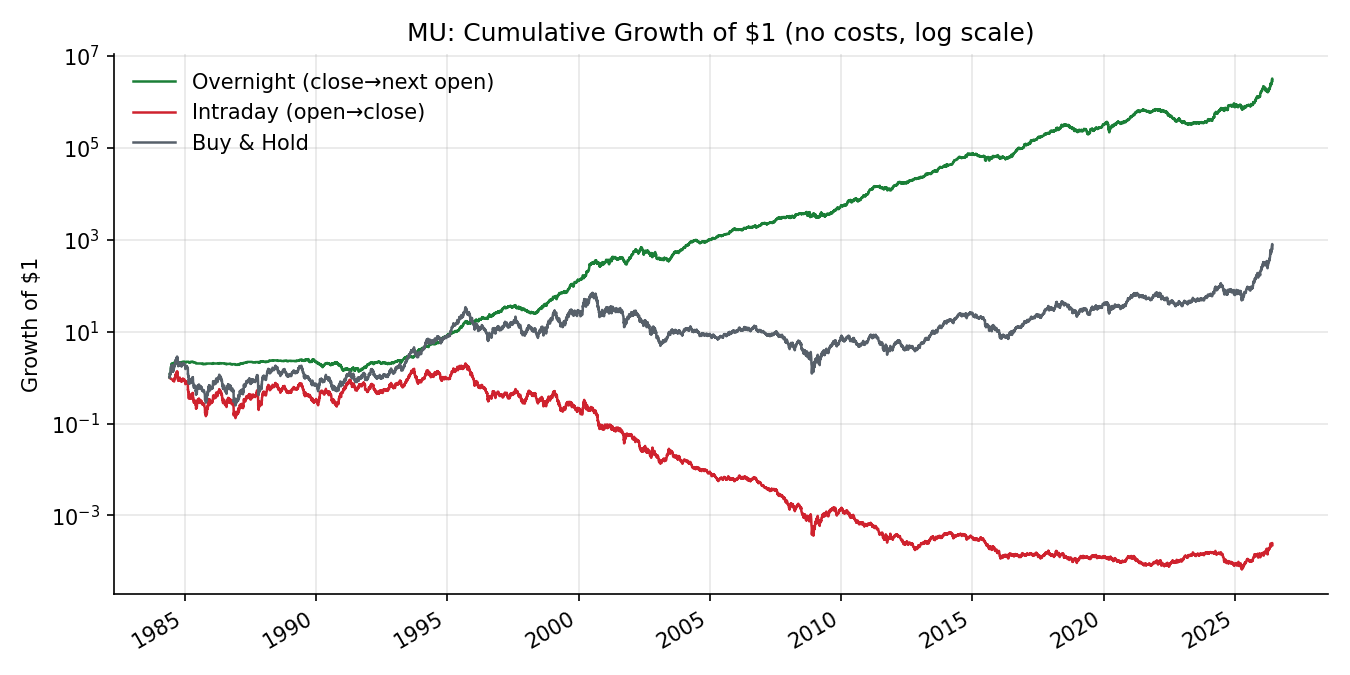
\includegraphics[width=\textwidth]{fig1_equity.png}
\caption{MU 三条腿累计净值（零成本，对数轴）。夜间腿 42 年累计 $2.8\times10^6$ 倍——即论文中天文数字的来源；日内腿累计归零；买入持有 640 倍恰为两者之积。}
\end{figure}

\begin{table}[H]\centering\small
\begin{tabular}{lrrrrrrrrr}
\toprule
策略 & 成本 & 日均(bps) & $t$ & Sharpe & Sortino & CAGR & 累计 & MaxDD & 胜率 \\
\midrule
夜间 & 0  & \pos{+15.6} & \pos{9.15} & 1.41 & 1.78 & \pos{+42.4\%} & 280万$\times$ & $-$54\% & 55.0\% \\
夜间 & 2  & \pos{+11.6} & \pos{6.80} & 1.05 & 1.39 & \pos{+28.8\%} & 4.07万$\times$ & $-$69\% & 46.1\% \\
夜间 & 5  & \pos{+5.6}  & \pos{3.27} & 0.50 & 0.67 & \pos{+10.7\%} & 71$\times$ & $-$89\% & 44.7\% \\
夜间 & 10 & \negv{$-$4.5} & \negv{$-$2.62} & $-$0.40 & $-$0.55 & \negv{$-$14.0\%} & 归零 & $-$100\% & 42.0\% \\
日内 & 0  & \negv{$-$2.4} & $-$0.73 & $-$0.11 & $-$0.17 & \negv{$-$18.1\%} & 归零 & $-$100\% & 46.1\% \\
买入持有 & --- & +13.4 & 3.61 & 0.56 & 0.84 & +16.6\% & 640$\times$ & $-$98\% & 48.5\% \\
\bottomrule
\end{tabular}
\caption{MU 绩效指标全表（1984--2026，成本单位为 bps/单边）。夜间腿日收益偏度 $+0.11$、峰度 $11.2$：厚尾显著，正态假设不成立。}
\end{table}

\subsection{回撤：夜间腿并非低风险}
\begin{figure}[H]\centering
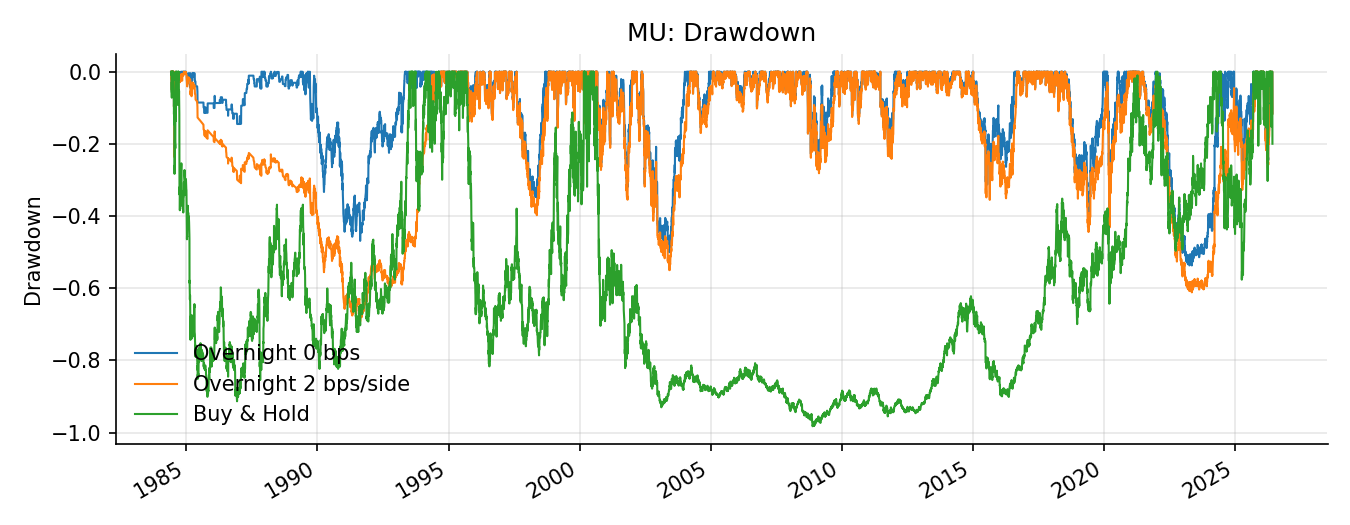
\includegraphics[width=\textwidth]{fig2_drawdown.png}
\caption{回撤曲线。夜间腿零成本最大回撤 $-54\%$，加 2 bps 成本后达 $-69\%$；"夜间稳赚"是错觉，它只是比买入持有（$-98\%$）的回撤浅。}
\end{figure}

\subsection{分年度：效应有大小年}
\begin{figure}[H]\centering
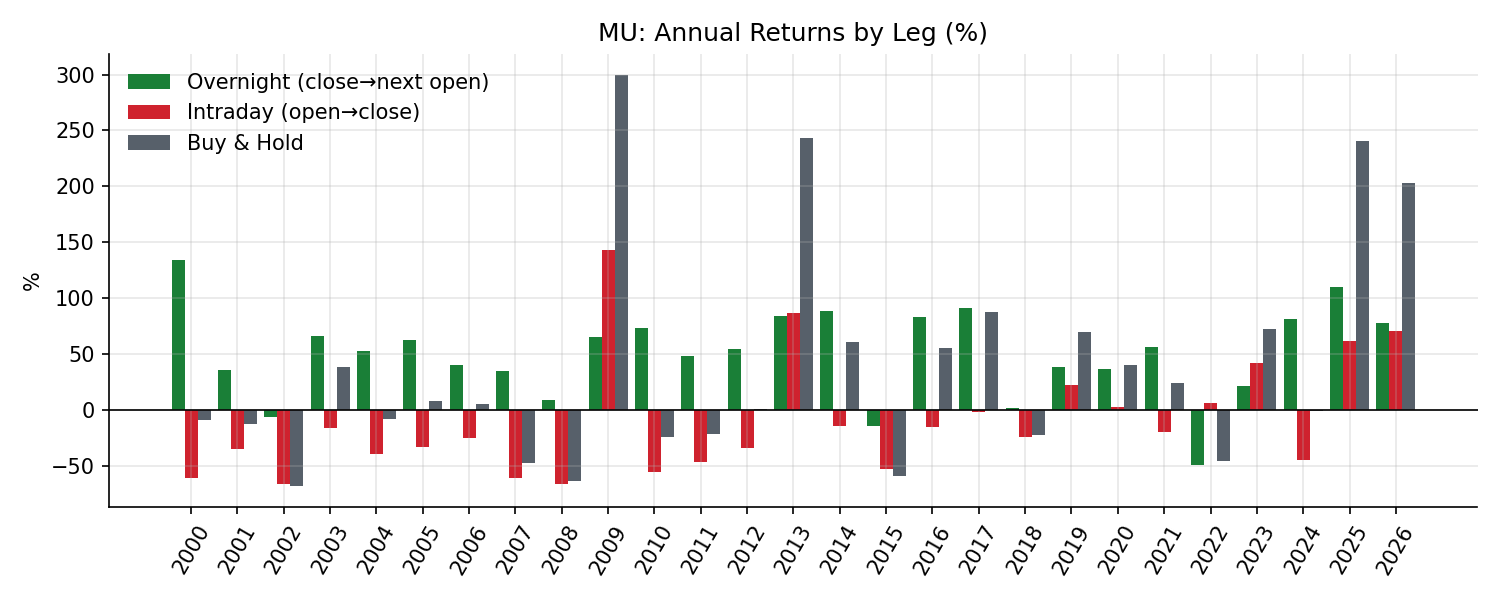
\includegraphics[width=\textwidth]{fig3_yearly.png}
\caption{2000 年以来分年度收益。注意 2022 年夜间腿 $-49\%$、2023 年日内腿反超——效应并非每年成立。2026 年为不完整年度（截至 6 月）。}
\end{figure}

%======================================================
\section{稳健性分析}
\subsection{滚动表现}
\begin{figure}[H]\centering
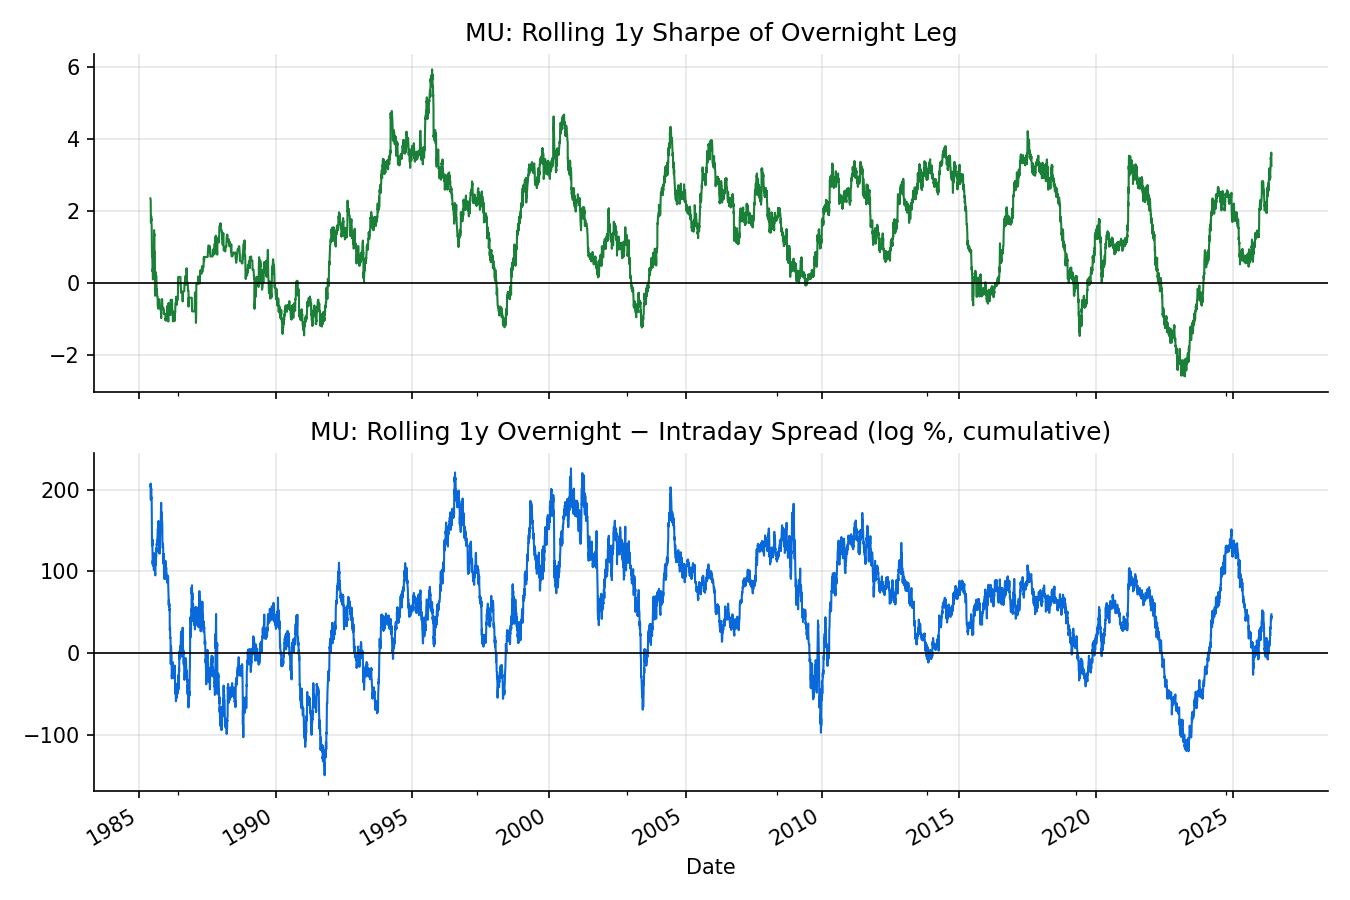
\includegraphics[width=\textwidth]{fig4_rolling.png}
\caption{上：夜间腿滚动 1 年 Sharpe，历史上 18.6\% 的时间为负；下：滚动 1 年"夜间$-$日内"累计价差（log \%），长期为正但 2022 年深度转负。}
\end{figure}

\subsection{月度与分布特征}
\begin{figure}[H]\centering
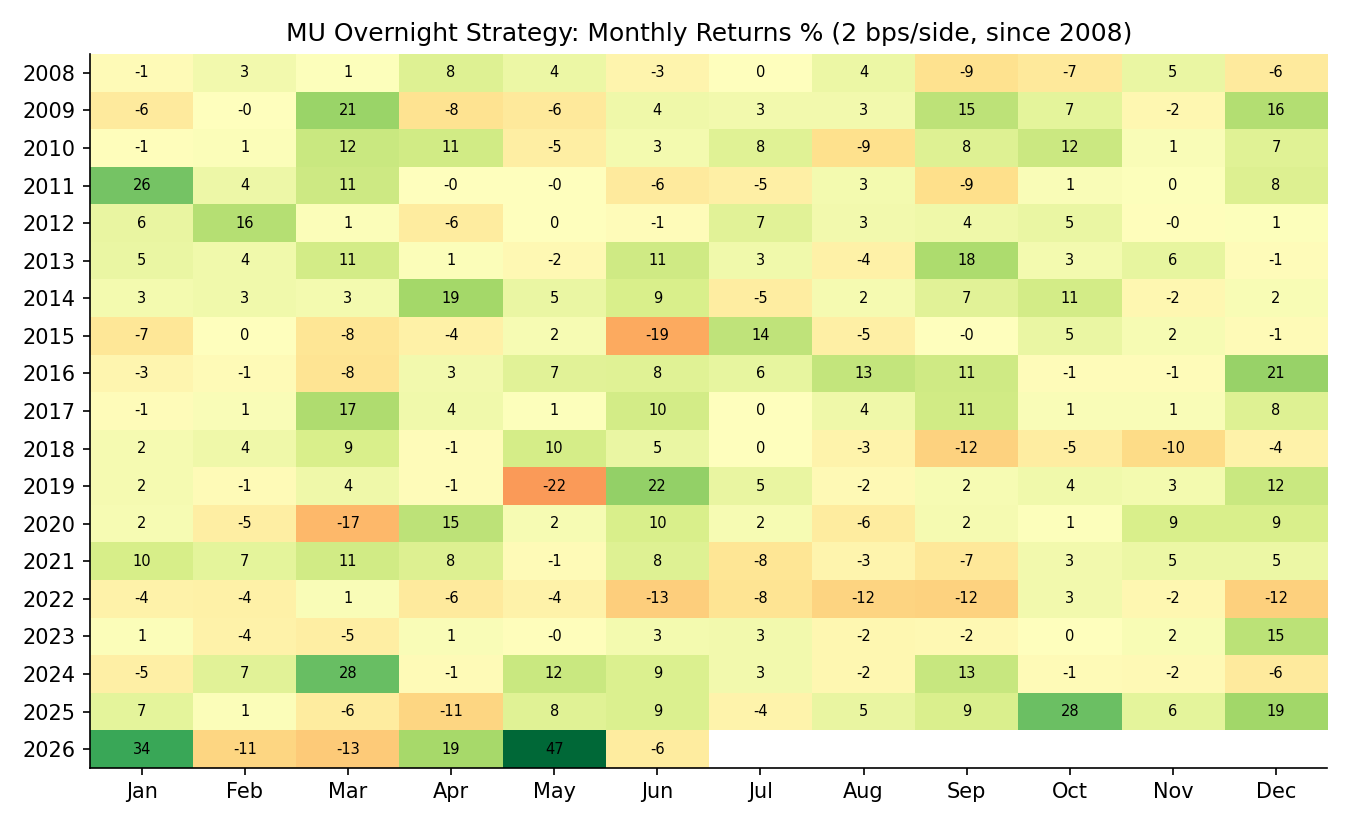
\includegraphics[width=0.95\textwidth]{fig5_heatmap.png}
\caption{夜间策略（2 bps/单边）月度收益热力图，2008 年至今。红色月份连片出现在 2008、2015、2018、2022——夜间腿在系统性风险期同样亏损，隔夜持仓承担跳空风险。}
\end{figure}

\begin{figure}[H]\centering
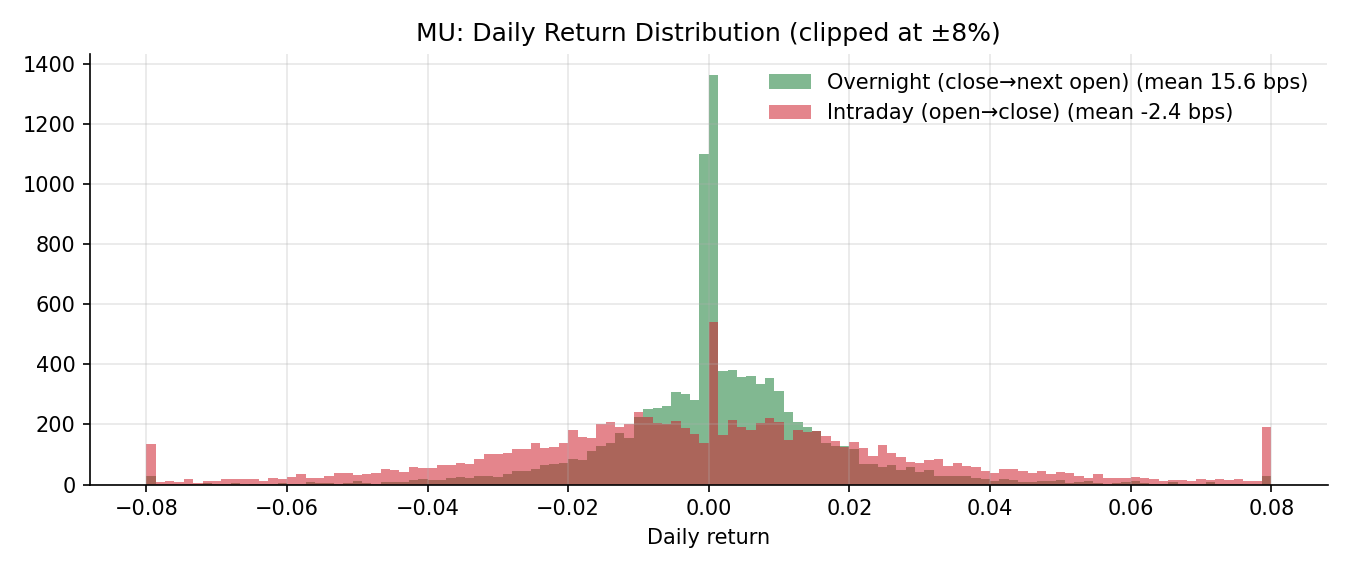
\includegraphics[width=\textwidth]{fig6_dist.png}
\caption{日收益分布对比。两个分布形状高度相似，差异在于均值的细微平移（$+15.6$ vs $-2.4$ bps）——肉眼不可见的日度优势，靠 42 年复利放大成天文数字。}
\end{figure}

%======================================================
\section{成本与可交易性：策略的生死线}
\begin{figure}[H]\centering
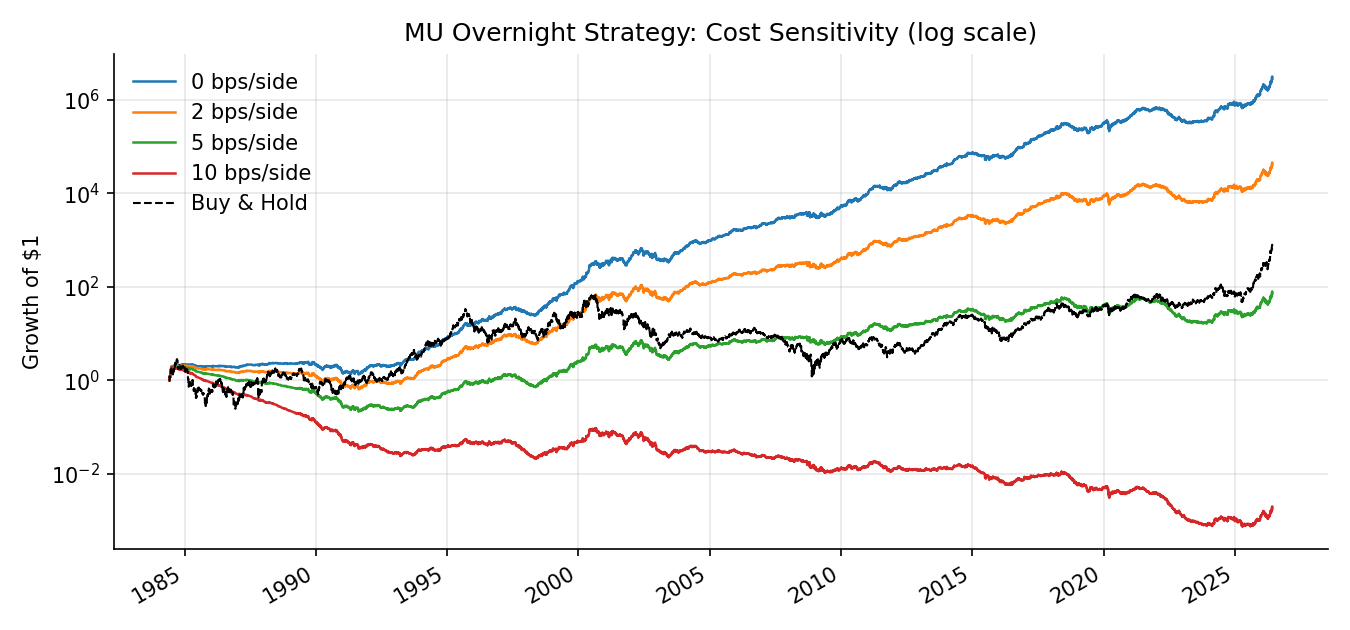
\includegraphics[width=\textwidth]{fig7_cost.png}
\caption{成本敏感性。0 bps 是神话，2 bps 仍跑赢买入持有，5 bps 落后于买入持有，10 bps 归零。盈亏平衡点 $\approx 15.6/2 = 7.8$ bps/单边。}
\end{figure}

\noindent 现实中的单边成本构成（美股零售）：
\begin{itemize}\itemsep0pt
  \item 佣金：0--1 bps（免佣券商为 0，但有订单流出售的隐性点差）；
  \item 开盘/收盘竞价滑点：\textbf{2--10 bps}（MU 这类票开盘跳空大，市价单更差）；
  \item 税务：每日翻仓全部为短期资本利得，按普通所得税率（最高 37\%），上表全部未计税。
\end{itemize}
\textbf{结论：用 MOO/MOC（开/收盘竞价单）执行可勉强压到 2--5 bps 区间，处于"勉强存活"与"死亡"之间；普通市价单执行必死。}

%======================================================
\section{需要持有多少天才能盈利？}
没有保证盈利的天数，只有随持有期上升的概率曲线：

\begin{figure}[H]\centering
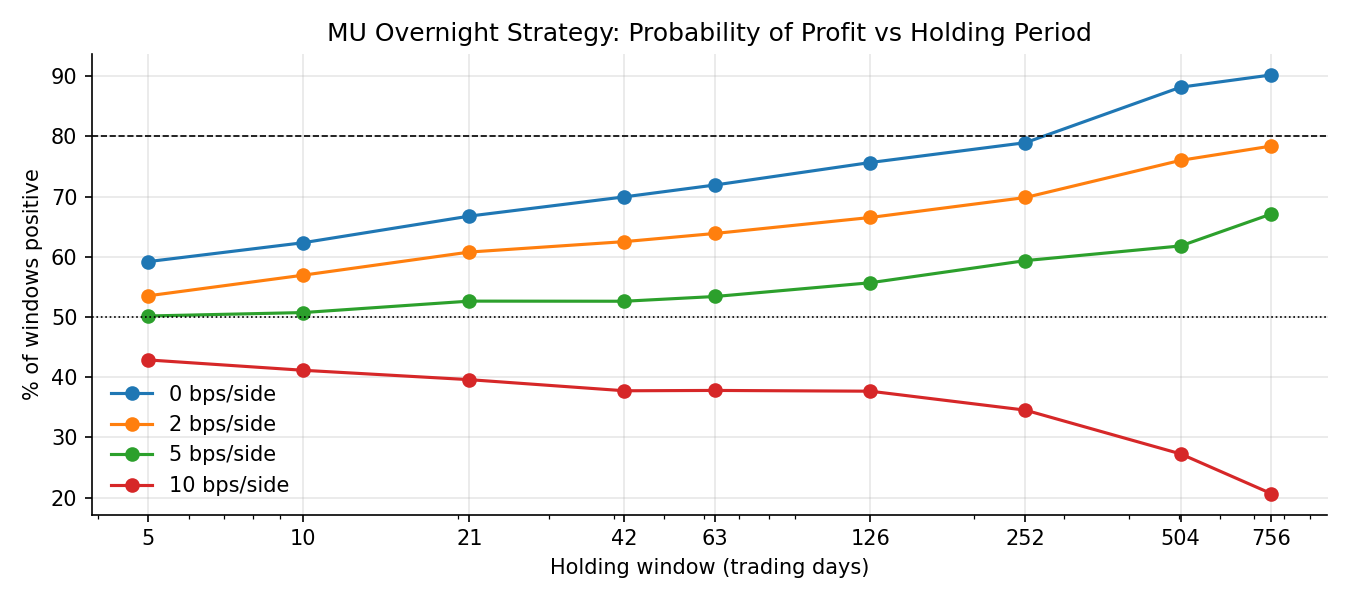
\includegraphics[width=\textwidth]{fig8_days_to_profit.png}
\caption{滚动 $N$ 日窗口累计收益为正的比例。虚线为 80\% 参考线：零成本需约 504 天（2 年）越过 88\%；2 bps 成本下 3 年仅 78\%；5 bps 成本下短期接近抛硬币。}
\end{figure}

\begin{table}[H]\centering\small
\begin{tabular}{lrrrrrr}
\toprule
持有窗口 & 21天 & 63天 & 126天 & 252天(1年) & 504天(2年) & 756天(3年) \\
\midrule
零成本   & 66.8\% & 71.9\% & 75.7\% & 79.0\% & \pos{88.2\%} & \pos{90.2\%} \\
2 bps/边 & 60.8\% & 63.9\% & 66.5\% & 69.8\% & 76.0\% & 78.4\% \\
5 bps/边 & 52.6\% & 53.4\% & 55.7\% & 59.4\% & 61.8\% & 67.1\% \\
\bottomrule
\end{tabular}
\caption{盈利概率表。最坏情形提醒：即使零成本，历史上也存在持有 3 年仍亏 $-42\%$ 的窗口（2021--2023）。}
\end{table}

%======================================================
\section{横截面：在什么股票上生效？}
\begin{figure}[H]\centering
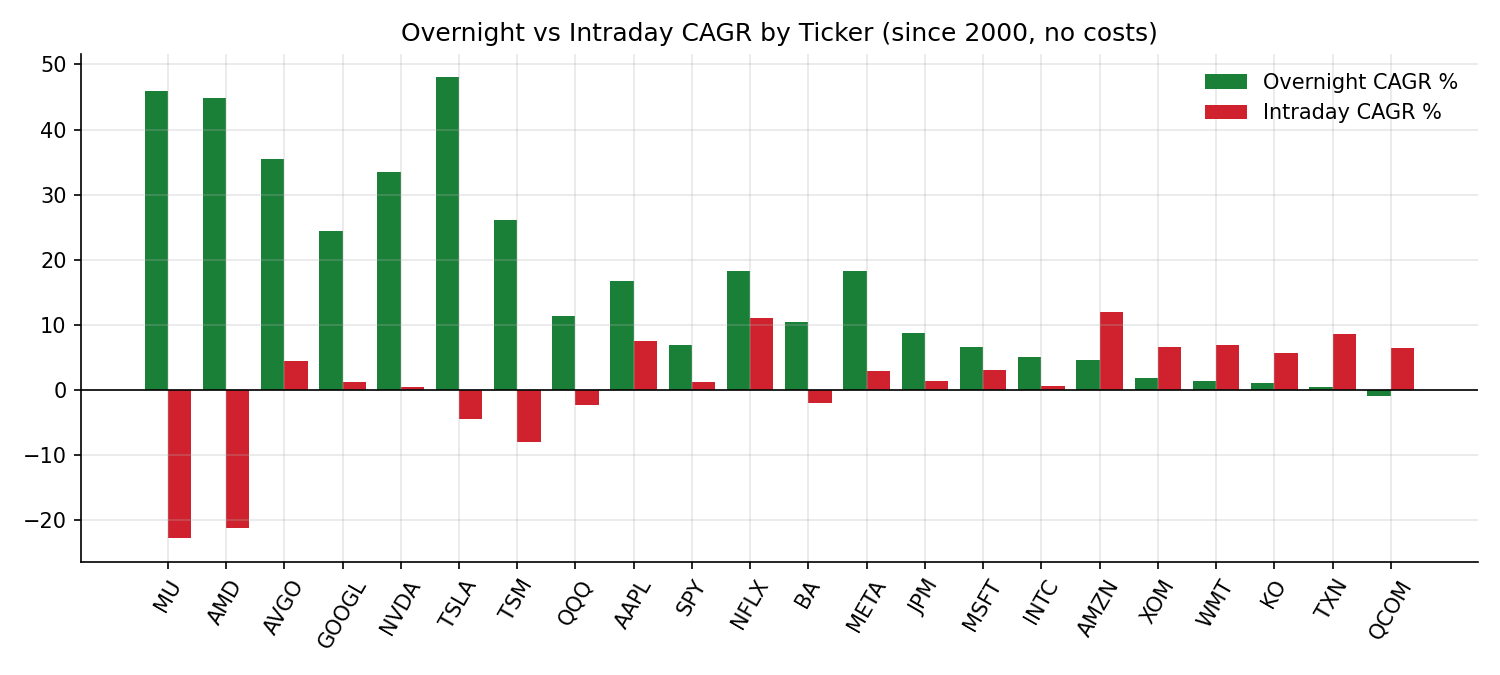
\includegraphics[width=\textwidth]{fig9_universe.png}
\caption{22 只标的夜间 vs 日内年化收益（2000 年起，零成本）。左侧绿柱压倒性领先的全部是高波动半导体/成长股；右端价值/防御股红柱反超。}
\end{figure}

\begin{table}[H]\centering\small
\begin{tabular}{lp{6.4cm}cc}
\toprule
分组 & 标的（夜间 $t$ 值） & 夜间CAGR范围 & 判定 \\
\midrule
强生效 ($t>5$) & MU(7.2) AMD(6.3) AVGO(5.9) GOOGL(5.6) & 24--48\% & \pos{显著} \\
              & NVDA(5.4) TSLA(5.2) TSM(5.1) & & \\
弱生效 ($2<t<5$) & QQQ AAPL SPY NFLX BA META JPM MSFT & 7--18\% & \pos{显著} \\
不生效 ($t<2$) & INTC AMZN XOM WMT KO TXN QCOM & $-1$--5\% & \negv{日内反超} \\
\bottomrule
\end{tabular}
\caption{横截面分组。22 票中 15 票夜间效应显著；不生效组中 AMZN/XOM/WMT/KO/TXN 的日内腿 $t>2$，方向完全反转。}
\end{table}

\begin{figure}[H]\centering
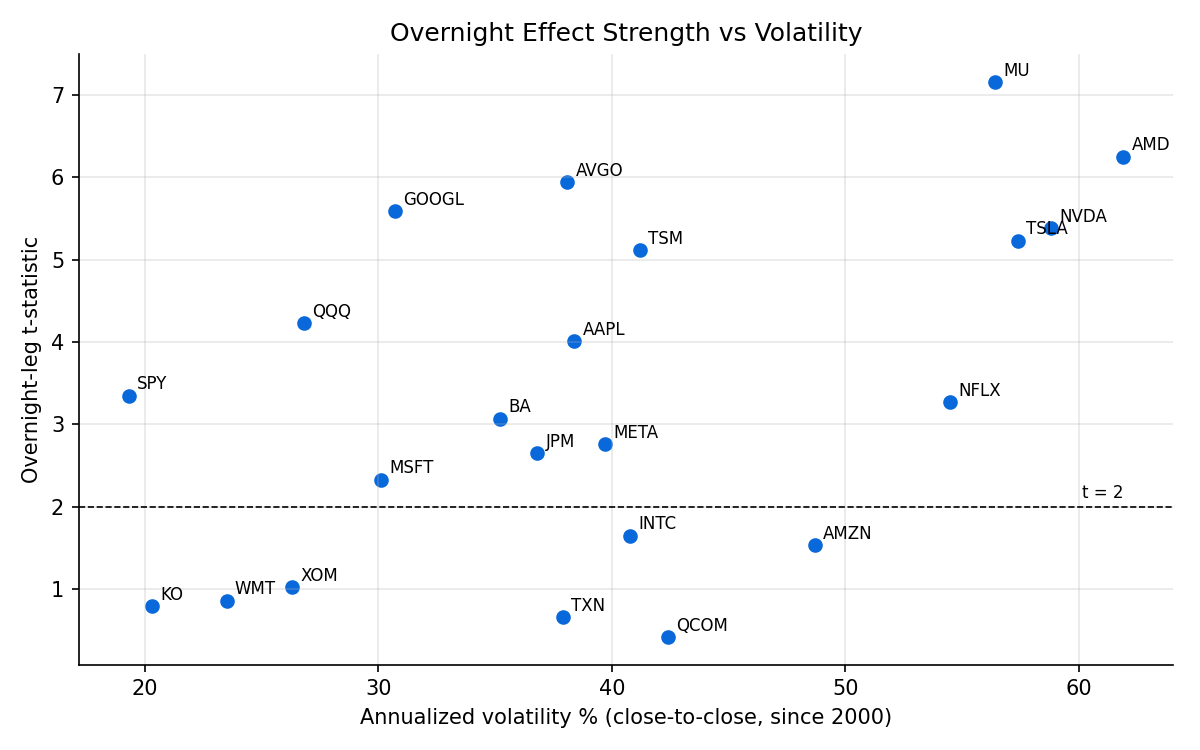
\includegraphics[width=0.8\textwidth]{fig10_scatter.png}
\caption{效应强度与波动率正相关（$\rho=0.51$）：波动率越高、散户关注度越高的股票，夜间效应越强——与 Lou--Polk--Skouras "拔河"机制（散户偏好开盘交易、机构偏好收盘交易）一致。}
\end{figure}

%======================================================
\section{市场状态分析：牛熊与涨跌下的表现}
\subsection{状态定义}
三个维度，全部用 $t-1$ 收盘可得信息判定，无前视偏差（样本统一自 2000 年起）：
\begin{itemize}\itemsep0pt
  \item \textbf{牛市/熊市}：SPY 收盘价高于/低于其 200 日均线（熊市天数占比 24.7\%）；
  \item \textbf{个股趋势}：该股收盘价高于/低于自身 200 日均线；
  \item \textbf{前日涨跌}：前一交易日总收益为正/负。
\end{itemize}

\subsection{MU：夜间收益集中在牛市与上升趋势中}
\begin{table}[H]\centering\small
\begin{tabular}{lrrrrrr}
\toprule
状态 & 天数 & 夜间均值(bps) & 夜间 $t$ & 夜间 Sharpe & 日内均值(bps) \\
\midrule
牛市 (SPY$>$MA200) & 4919 & \pos{+20.3} & \pos{8.58} & \pos{1.94} & $-$7.9 \\
熊市 (SPY$<$MA200) & 1727 & +7.1 & 1.17 & 0.45 & $-$0.5 \\
自身上升趋势 & 3518 & \pos{+23.1} & \pos{7.99} & \pos{2.14} & --- \\
自身下降趋势 & 3128 & +9.8 & 2.57 & 0.73 & --- \\
前一日上涨 & 3322 & \pos{+21.2} & \pos{6.36} & 1.75 & --- \\
前一日下跌 & 3324 & +12.5 & 3.76 & 1.03 & --- \\
\bottomrule
\end{tabular}
\caption{MU 夜间腿条件统计（2000 年起，零成本）。牛市夜间收益是熊市的近 3 倍且唯一高显著；自身趋势过滤效果最强：上升趋势中 Sharpe 达 2.14。}
\end{table}

\begin{figure}[H]\centering
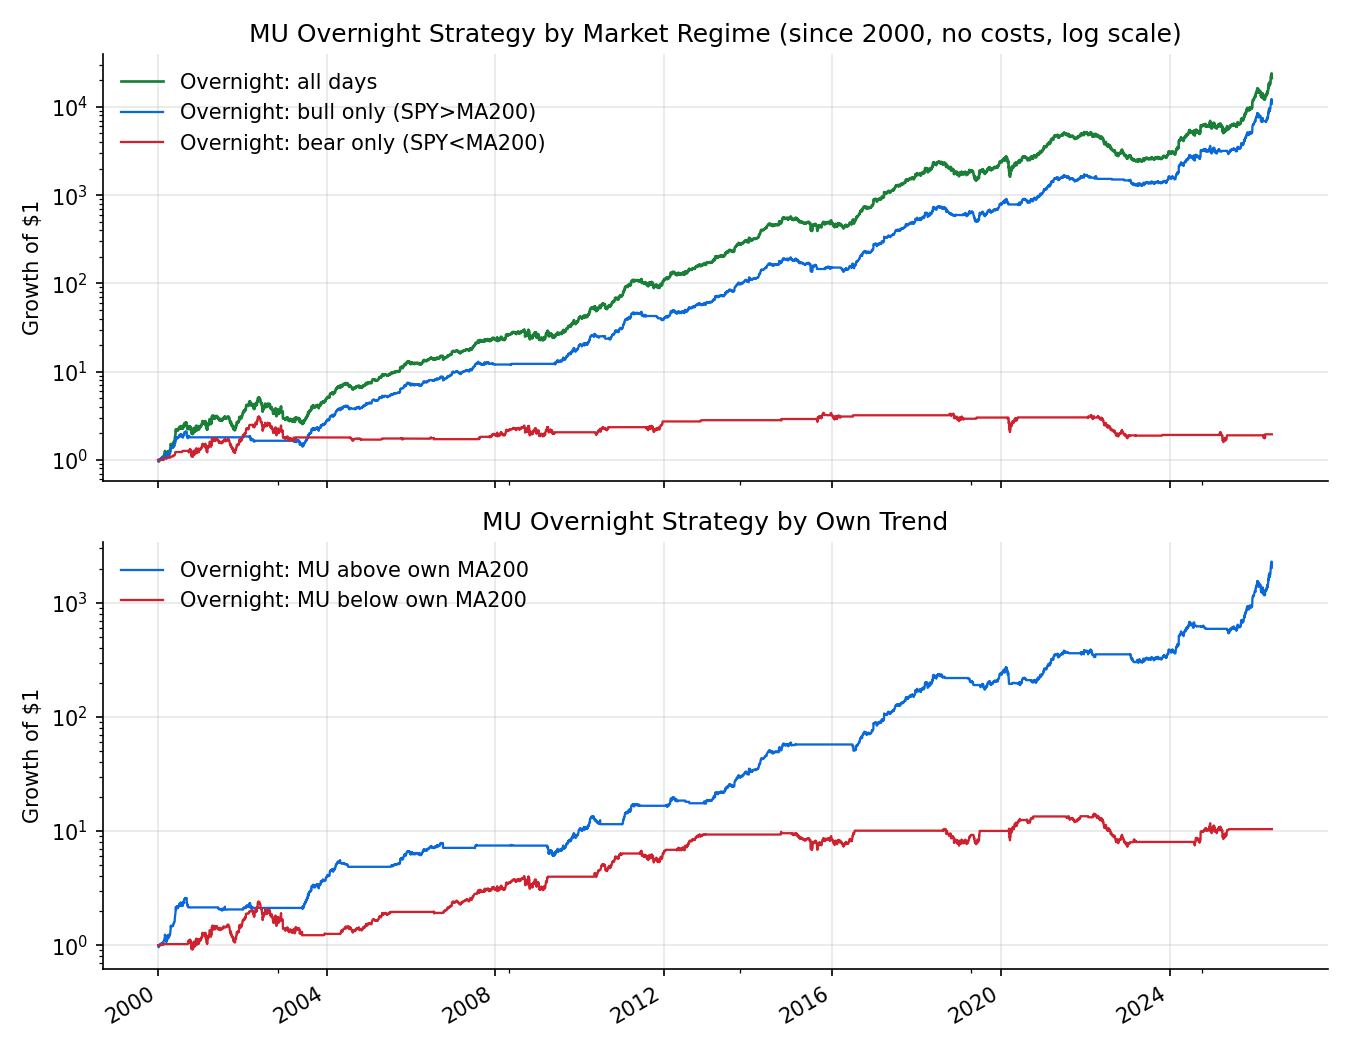
\includegraphics[width=0.92\textwidth]{fig11_regime_equity.png}
\caption{MU 夜间策略按状态拆分的累计净值（对数轴）。上图：牛市贡献了绝大部分收益，熊市段净值近乎走平；下图：自身趋势过滤的区分度更高——趋势下方时段几乎不贡献收益却贡献大量回撤。}
\end{figure}

\begin{figure}[H]\centering
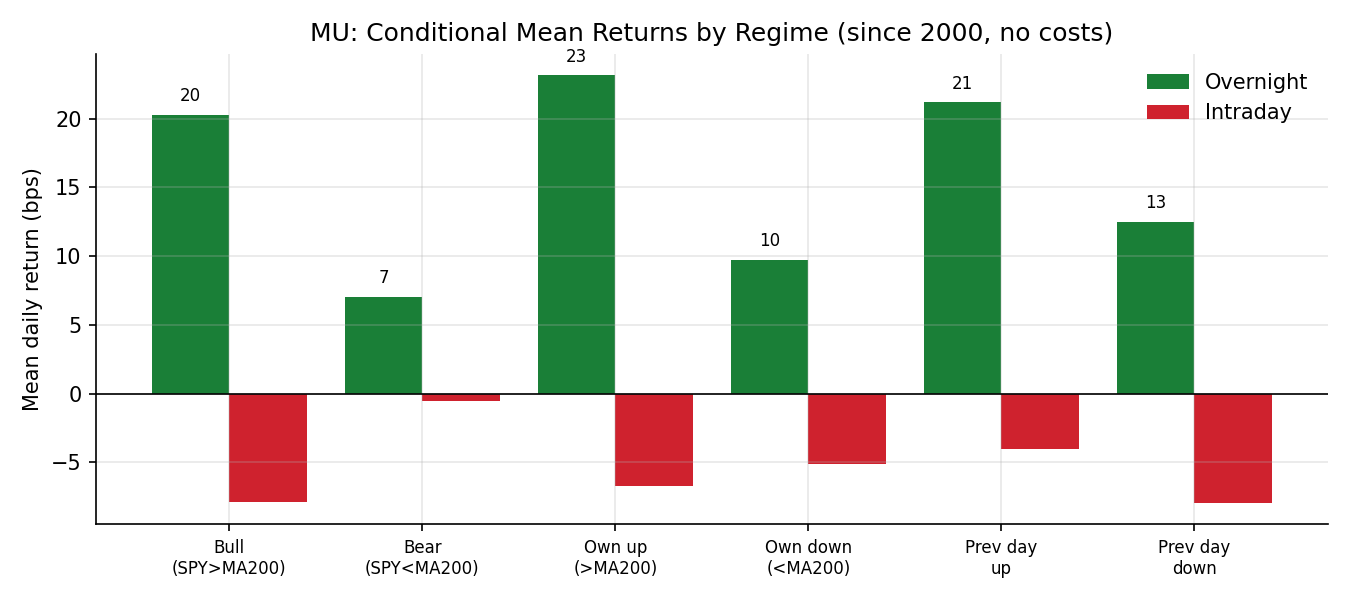
\includegraphics[width=0.92\textwidth]{fig14_mu_conditional.png}
\caption{MU 六种状态下的夜间 vs 日内日均收益。所有状态下夜间均为正、日内均为负或近零——方向不变，但幅度由市场状态决定。}
\end{figure}

\subsection{横截面：熊市中效应整体崩塌}
\begin{table}[H]\centering\small
\begin{tabular}{lcccc}
\toprule
状态 & 夜间均值(bps, 22票平均) & 为正票数 & 显著票数 ($t>2$) & 日内均值(bps) \\
\midrule
牛市 & \pos{+8.6} & 22/22 & \pos{18/22} & +0.7 \\
熊市 & +2.1 & 13/22 & \negv{1/22} & \pos{+7.6} \\
自身上升趋势 & +7.6 & 18/22 & 13/22 & --- \\
自身下降趋势 & +5.6 & 19/22 & 8/22 & --- \\
前一日上涨 & +7.3 & 18/22 & 12/22 & --- \\
前一日下跌 & +6.7 & 22/22 & 9/22 & --- \\
\bottomrule
\end{tabular}
\caption{22 票横截面的状态汇总。牛熊差异远大于其他维度：熊市中唯一显著的是 AMD（$t=2.85$），且 NVDA、TSM、AAPL、AMZN、NFLX 等 9 票夜间均值转负，而日内腿平均反超至 $+7.6$ bps。}
\end{table}

\begin{figure}[H]\centering
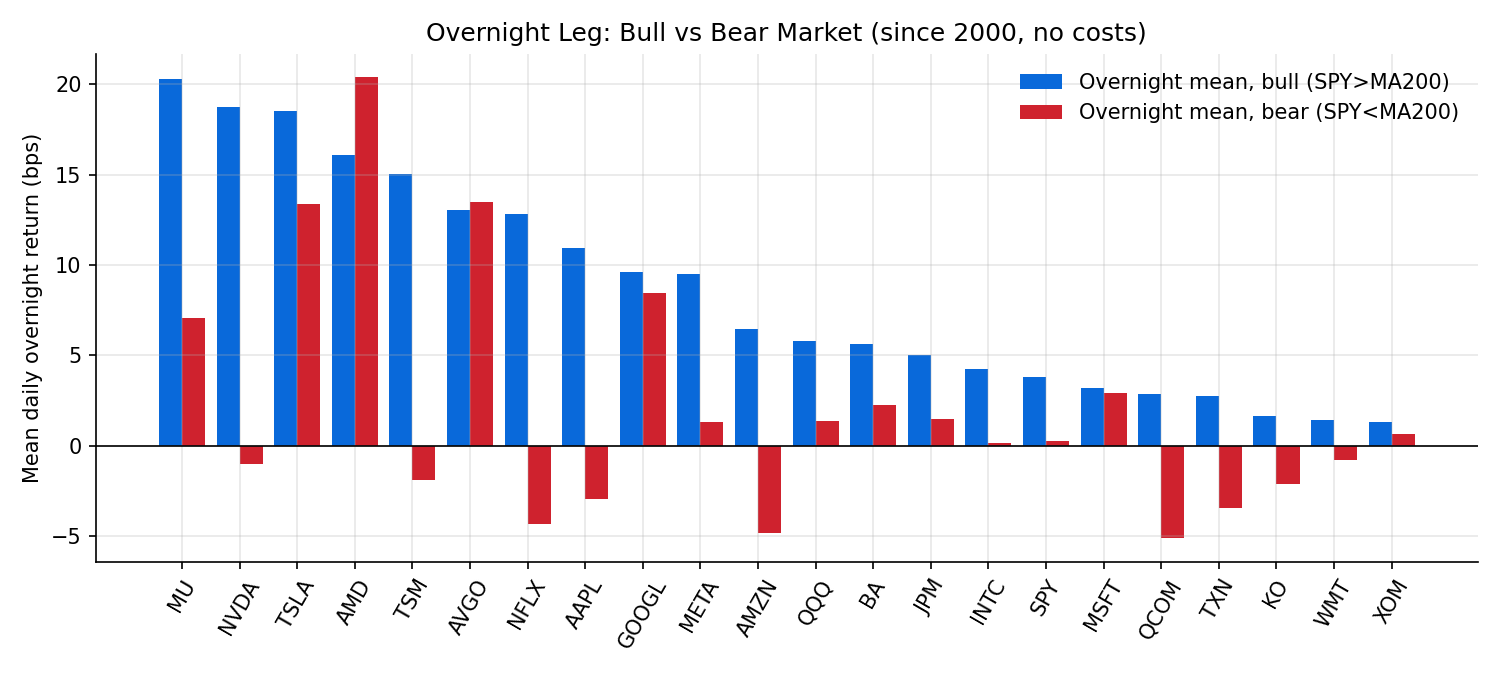
\includegraphics[width=\textwidth]{fig12_bull_bear.png}
\caption{各标的牛市 vs 熊市夜间日均收益。蓝柱（牛市）几乎全部显著为正；红柱（熊市）杂乱无章——熊市中的夜间收益在统计上与零无异。}
\end{figure}

\begin{figure}[H]\centering
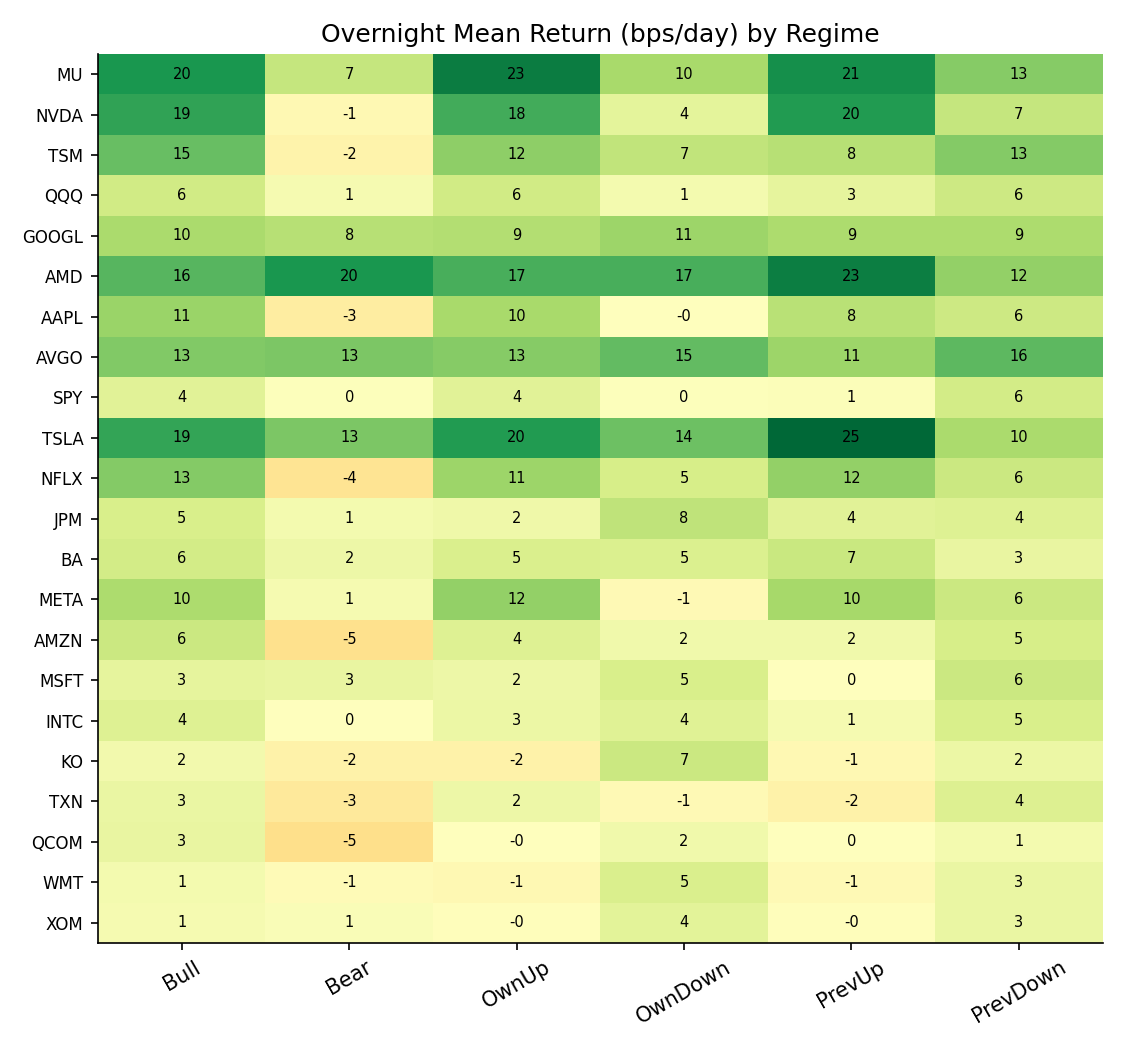
\includegraphics[width=0.78\textwidth]{fig13_regime_heatmap.png}
\caption{状态 $\times$ 标的热力图（夜间日均 bps）。左侧两列（牛/熊）色差最大，验证市场状态是夜间效应的第一决定因素。}
\end{figure}

\subsection{机制解读与策略含义}
\begin{itemize}\itemsep2pt
  \item \textbf{夜间收益的本质更接近"牛市里的隔夜风险溢价"}：牛市中隔夜消化的信息以利好为主，承担跳空风险获得补偿；熊市中隔夜跳空以利空为主，溢价消失甚至反转。
  \item \textbf{"拔河"方向在熊市掉头}：散户开盘追买的行为在牛市推高开盘价（利好夜间腿），熊市中开盘恐慌抛售反而压低开盘价，让日内腿（低开后盘中修复）受益——这解释了日内腿熊市均值 $+7.6$ bps 的反超。
  \item \textbf{可操作的改进}：给夜间策略加趋势过滤（仅在个股位于自身 MA200 上方时交易），MU 的 Sharpe 从 1.39（2000 年起全样本）升至 2.14，同时避开 2022 式 $-49\%$ 的年度回撤——代价是约 47\% 的时间空仓。
  \item \textbf{风险提示}：牛熊判定基于 MA200 是滞后指标，状态切换初期（如 2020 年 3 月、2022 年 1 月）仍会吃到最剧烈的隔夜跳空。
\end{itemize}

%======================================================
\section{结论与下一步}
\subsection{四个问题的最终答案}
\begin{enumerate}\itemsep2pt
  \item \textbf{在 MU 上生效吗？} 生效，$t=9.15$ 在统计上无可辩驳；但 280 万倍是零成本神话，2 bps 下缩水到 4 万倍，5 bps 下不如买入持有。
  \item \textbf{多少天能盈利？} 无保证。零成本约 2 年达 88\% 概率；现实成本下 3 年也只有 $\sim$78\%，且存在 3 年亏 40\% 的历史窗口。
  \item \textbf{什么股票生效？} 高波动成长/半导体股（MU、AMD、NVDA、TSLA、AVGO、TSM 等）；价值/防御股不生效甚至反向。
  \item \textbf{牛熊表现？} 效应本质上是牛市现象：牛市 18/22 票显著、熊市仅 AMD 幸存且 9 票转负；日内腿在熊市反超。最有效的单一改进是趋势过滤（个股 $>$ MA200 才交易，MU 的 Sharpe 1.39 $\to$ 2.14）。
  \item \textbf{怎么用？} 不建议作为独立策略；建议作为\textbf{执行时点优化}——本来要买的票放收盘买、要卖的放开盘卖，把异象当免费顺风。
\end{enumerate}

\subsection{升级到"可交易级"回测还需要}
\begin{enumerate}\itemsep2pt
  \item 分钟级数据：用开/收盘前后 5 分钟 VWAP 替代理想价，实测滑点；
  \item MOO/MOC 竞价单模拟（事件驱动框架，如 LEAN）；
  \item 税务模型（短期资本利得）与融资成本；
  \item 组合化：等权一篮子高波动半导体股，替代单票 MU 以降低过拟合；
  \item 样本外验证：2020 年前定参、2020 年后验证，重点检查 2022 式反转。
\end{enumerate}

\appendix
\section{局限性声明}
\begin{itemize}\itemsep0pt
  \item 开盘价/收盘价成交为理想化假设，真实可成交价更差；
  \item Yahoo Finance 早年数据可能存在开盘价质量问题（部分 90 年代前数据开盘价为复制值）；
  \item 单票分析存在选择偏差——MU 正是因为效应极端才被论文选中；
  \item 横截面样本为手选 22 票，非全市场扫描；
  \item 未考虑停牌、退市、流动性枯竭情形；2026 年为不完整年度。
\end{itemize}

\vspace{1em}
\noindent\small 数据与代码：\texttt{research/overnight/}（\texttt{backtest\_overnight.py}、\texttt{make\_report\_assets.py}）。
参考文献：Lou, Polk, Skouras (2019), \textit{A Tug of War: Overnight versus Intraday Expected Returns}, JFE.
\end{document}
